\documentclass{article}
\usepackage[utf8]{inputenc}

\title{
MCU-Fortifier User Manual
}
\author{
  Security Embedded\\
  \texttt{}
  \and
  Daniele Giuliani (DG)\\
  \texttt{daniele.giuliani@unitn.it}
}
\date{December 2021}

\usepackage{natbib}
\usepackage{graphicx}
\usepackage{listings}
\usepackage{color}

\definecolor{dkgreen}{rgb}{0,0.6,0}
\definecolor{gray}{rgb}{0.5,0.5,0.5}
\definecolor{mauve}{rgb}{0.58,0,0.82}

\lstset{frame=tb,
  language=C,
  aboveskip=3mm,
  belowskip=3mm,
  showstringspaces=false,
  columns=flexible,
  basicstyle={\small\ttfamily},
  numbers=none,
  numberstyle=\tiny\color{gray},
  keywordstyle=\color{blue},
  commentstyle=\color{dkgreen},
  stringstyle=\color{mauve},
  breaklines=true,
  breakatwhitespace=true,
  tabsize=3
}

\usepackage{fancyhdr}
\pagestyle{fancy}
\fancyhead{}
\renewcommand{\headrulewidth}{0pt}
\fancyfoot{}
\fancyfoot[C]{\thepage}           % page number Center Even, Center Odd
\fancyfoot[R]{Revision 1.2}
\fancyfoot[L]{Confidential}

\usepackage{vhistory}
\usepackage{hyperref}

\begin{document}

\maketitle
\newpage
% beginning revision table
\begin{versionhistory}
	\vhEntry{1.0}{09/10/2021}{DG}{Created first version}
	\vhEntry{1.1}{03/11/2021}{DG}{Switching to STM32L475 MCU, update MCU-Foritifier Configuration, update Fortification process with new makefile configuration and memory map, add Update Server communication protocol and configuration}
	\vhEntry{1.2}{28/12/2021}{DG}{Update compilation process, add Microvisor self-update capabilities, add Microvisor Activation section, update all screenshot, miscellaneous fixes}
	%\vhEntry{1.2}{03/02/04}{Author1|Author2}{Changes description}
\end{versionhistory}

\newpage
% beginning table of content
\tableofcontents
\newpage

% beginning manual
\section{Scope of document}
This document is targets developers that want to use MCU-Fortifier in order to increase the security of their devices. 

\section{Introduction}
MCU-Fortifier is a solution for memory isolation that increases the security of embedded devices. In particular, MCU-Fortifier is designed to work with Cortex M3 devices equipped with a Memory Protection Unit (MPU).

The MCU-Fortifier solution is composed of 4 distinct parts:
\begin{itemize}
    \item A \textit{Fortified Application}: an embedded application specifically compiled in order to be compatible with MCU-Fortifier.
    \item The \textit{MCU-Fortifier Microvisor}: the first piece of software executed on boot of the embedded device, acts as an OS, bootstraps the execution of the Fortified Application and constantly monitors it.
    \item An \textit{Instrumenter}: a tool used during the compilation process that allows the creation of fortified applications.
    \item An \textit{Update Server}: a server application running on a more powerful machine capable of providing secure updates and error reporting capabilities to boards running the MCU-Fortifier Microvisor.
\end{itemize}

\section{MCU-Fortifier Design}
MCU-Fortifier is design to protect the device by isolating the untrusted Fortified Application form the trusted MCU-Fortifier Microvisor. This is done by using a feature of the ARMv7 Architecture that allows the execution of code in two different modes: \textit{privileged} and \textit{unprivileged}.

While the Microvisor can execute both in privilege or unprivileged mode, the Fortified Application is only allowed to execute in unprivileged mode which prevents it form escaping the memory isolation and ACP imposed by the Microvisor through the use of the MPU.

\section{Configuring MCU-Fortifier}
The source files \textit{microvisor\_config.h} and \textit{microvisor\_config.c} are designed to be modify by the user in order to customize the Microvisor configuration. These files contain the following:
\begin{itemize}
	\item Network parameters, such as Wi-Fi SSID and password necessary for connecting the device.
	\item Connection parameters, such as the IP and port of the remote Update Server that will be queried for updates on boot.
	\item Symmetric encryption key, used to encrypt and authenticate the communication with the Update Server (must be set to the same value for both the Microvisor and the Update Server).
	\item MCU-Fortifier License, used to activate the device during the first boot by communicating with the Activation Server (see Section \ref{sec:microvisor_activation} for more information).
\end{itemize}

The other main file that can be customized is \textit{stm32l475vg\_mpu.c} which contains the Memory Protection Unit configuration. In most circumstances the default configuration provided with the release of MCU-Fortifier will suffice. More advanced user can modify this file to fine tune the behavior of the MPU.

\section{Compiling MCU-Fortifier Microvisor}
\label{sec:microvisor_compile}
The process of obtaining the MCU-Fortifier Microvisor executable is straight forward.
\begin{itemize}
    \item Open the release folder of \textit{MCU-Fortifier}.
    \item Edit the \verb|GCC_PATH| and \verb|PREFIX| variables inside the \textit{Makefile} in order to point to the installation of GNU Arm Embedded Toolchain on your system.
    \item Open a terminal and type ``\verb|make|``.
\end{itemize}
If the compilation process was successful, the executable can be found in the \textit{Build} folder under the name \textit{MCU-Fortifier.elf}.

\subsection{Notes for Windows Users}
\paragraph{PowerShell}
On Windows the equivalent of the Linux terminal are \textit{CMD} and \textit{PowerShell}. To open them a folder make sure that no files are selected then, while holding \textit{Shift}, right click on the empty space in the folder and select ``Open PowerShell window here''.

\paragraph{GNU Arm Embedded Toolchain}
The  GNU Arm Embedded Toolchain is installed automatically together with STM32CubeIDE inside the \textit{plugin} folder. The path will vary depending on the version of STM32CubeIDE and GNU Arm Embedded Toolchain but it will generally look as such:
\begin{verbatim}
C:\ST\STM32CubeIDE_1.7.0\STM32CubeIDE\plugins\com.st.stm32cube
    .ide.mcu.externaltools.gnu-tools-for-stm32.9-2020-q2-update
    .win32_2.0.0.202105311346\tools\bin
\end{verbatim}

\paragraph{Makefile Paths}
Given that \textit{make} is a program originally designed for Linux, when editing the \textit{Makefile} ensure that the paths are specified with forward slashes instead of back slashes (e.g. \verb|C:/Correct/Forward/Slash/Path| instead of \verb|C:\Wrong\Back\Slash\Path|). Also, if a directory or a file inside a path contains a white space it will need to be escaped by using a back slash (e.g. \verb|C:/My Folder/file.exe| becomes \verb|C:/My\ Folder/file.exe|).

\paragraph{Make Tools}
\label{ref:make_tools}
In addition to the GNU Arm Embedded Toolchain, STM32CubeIDE also provides \textit{make} and a series of commonly used commands on Linux (e.g. \textit{mkdir}, \textit{sh}, \textit{rm}). In order for \textit{make} to access these commands the Windows \verb|Path| environment variable must be updated with the directory containing them. This can be done with the following steps:
\begin{itemize}
    \item Open \textit{My Computer}.
    \item Right click on an empty space and select \textit{Properties}.
    \item In the left-most section of the newly opened window, click on \textit{Advanced System Settings}.
    \item At the bottom, click on \textit{Environment Variables}.
    \item Select either the System Variable or User Vairable \verb|Path| and click \textit{Edit}.
    \item Append at the bottom a new entry with the directory containing the Make Tools.
\end{itemize}

STMCube IDE will install the Make Tools in the plugin directory, an example of path will look as follows:
\begin{verbatim}
C:\ST\STM32CubeIDE_1.7.0\STM32CubeIDE\plugins\com.st.stm32cube
    .ide.mcu.externaltools.make.win32_2.0.0.202105311346
    \tools\bin
\end{verbatim}

\paragraph{Python} Python is a necessary in order to create fortified applications compatible with MCU-Fortifier. While this software is already installed in most Unix-like OSes, Windows user will be required to install it manually. During the installation an option to add Python to the Path environment variable will be displayed. It is advised to perform this operation in order to avoid having to configure additional paths later on.


\section{MCU-Fortifier Microvisor Activation}
\label{sec:microvisor_activation}
In order execute correctly MCU-Fortifier must be activated. The activation is a one-time process performed on the first boot of MCU-Fortifier.

In order to completely correct the activation the device must be capable of communicating with the Security Embedded Activation Server, for this reason a valid Internet connection is required on the first boot. Subsequent boots check that the activation has been performed without requiring any Internet access.

A board that has not been activated will continue rebooting and attempt to connect to Internet until the activation process has been carried out successfully. If your fortified application is not being executed, make sure that a valid license is specified in the \textit{microvisor\_config.c} file.


\section{Fortifying an Application}
This section will explain how to setup the IDE in order turn any standard project into a Fortified Application and execute it under the supervision of the MCU-Fortifier Microvisor. This example utilizes a B-L475E-IOT01A1 board (STM32L475VG MCU) and shows the steps in order to configure STM32CubeIDE as the development environment.

\subsection{Blinky Application}
For the user convenience, every release of MCU-Fortifier provides a sample Blinky application already fortified that can be imported directly into STM32CubeIDE but the following example can useful to familiarize with the toolchain. As a sidenote, in some occasion STM32CubeIDE will discard the build and launch configuration (e.g. content of the \textit{Debug} folder) when importing a project, in this case it is necessary to manually copy the missing content and disable the automatic building process again.
\begin{itemize}
    \item Begin by creating a new STM32 Project in STM32CubeIDE, select the STML475VG board and name it. In this example we will create an application that makes the led on the board blink and will name it \textit{blinky\_l475}.
    \item In the Device Configuration screen, left click on pin \verb|PB14|, \verb|PC9| and configure them as \verb|GPIO_Output| as shown in Figure \ref{fig:led_config}. In the GPIO Configuration tab assign a label to each of the pins, respectively \verb|Green_Led| and \verb|Network_Led|.
    \item Now open the source file \verb|main.c| and edit the \verb|main()| function in order to make the leds blink as in Listing \ref{lst:main}.
\end{itemize}

\begin{figure}
\centering
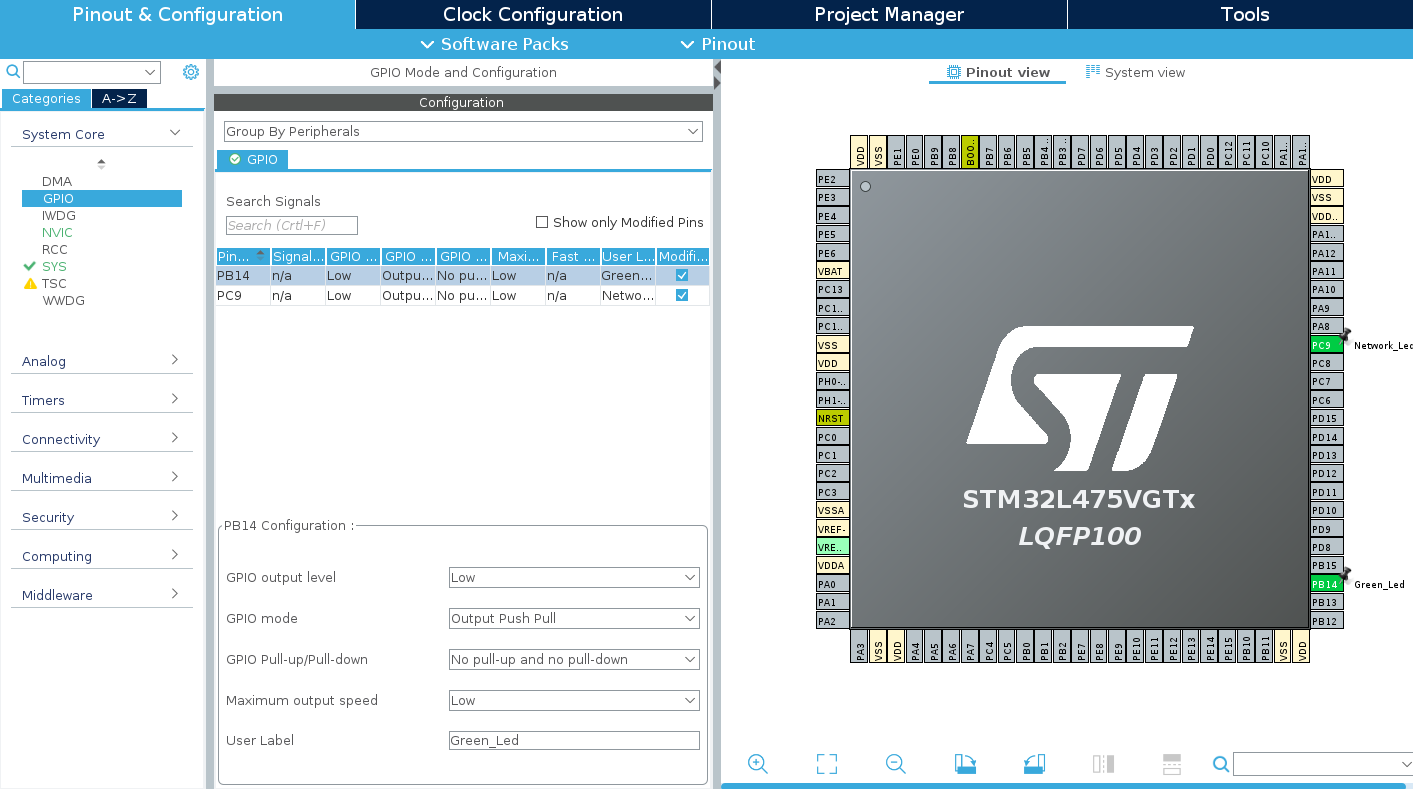
\includegraphics[scale=.25]{images/led_config.png}
\caption{Pin configuration for led use on STM32L475VG board}
\label{fig:led_config}
\end{figure}

\begin{lstlisting}[caption={modified main.c file},captionpos=b,label=lst:main]
int main(void)
{
  /* Reset of all peripherals, Initializes the Flash interface and the Systick */
  HAL_Init();
  
  /* Configure the system clock */
  SystemClock_Config();
  
  /* Initialize all configured peripherals */
  MX_GPIO_Init();
  
  /* Led blink */
  while (1)
  {
    HAL_GPIO_TogglePin(Green_Led_GPIO_Port, Green_Led_Pin);
    //HAL_GPIO_TogglePin(Network_Led_GPIO_Port, Network_Led_Pin);
    HAL_Delay(100);
  }
}
\end{lstlisting}

\begin{itemize}
    \item Build the application, and launch a Debug session with the default Debug configuration.
    \item Verify that the application is working as intended (the green led should be blinking).
\end{itemize}


\subsection{Customize Build Process}
To generate a Fortified Application the build process must be configured in order to run the \textit{Instrumenter} on the source files. STM32CubeIDE uses \textit{make} to drive the build process so \verb|Makefile| responsible for the build process must be modified in order to run the instrumentation. 

\begin{itemize}
    \item Begin by right clicking on the \textit{blinky\_l475} project and going on \textit{Properties}.
    \item Under the \textit{C/C++ Build} tab uncheck the \textit{Generate Makefiles automatically} option as shown in Figure \ref{fig:auto_make}. Click on \textit{Apply and Close}.
    \item In the project tree, open the Debug folder (the folder will only be present after the first build performed in the previous steps).
\end{itemize}

\begin{figure}
\centering
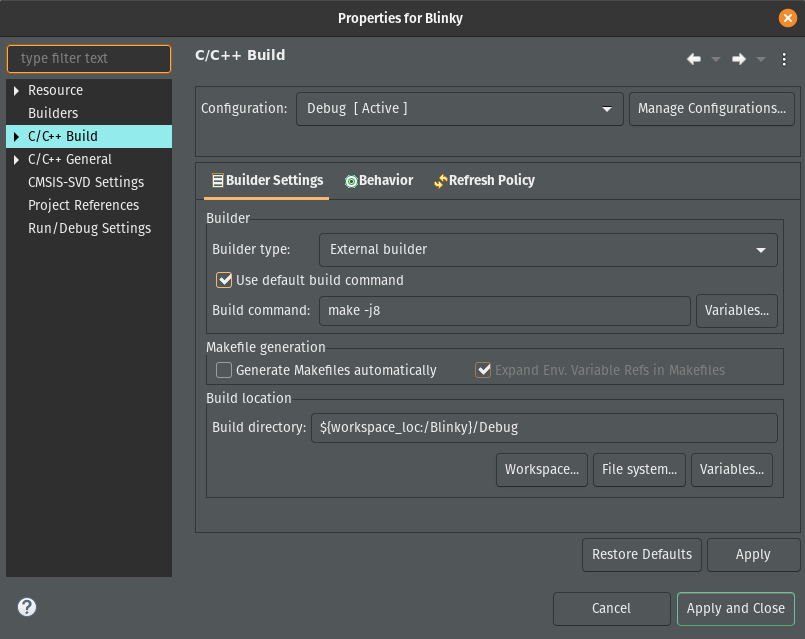
\includegraphics[scale=.4]{images/auto_make.png}
\caption{Project build configuration}
\label{fig:auto_make}
\end{figure}

\subsubsection{Makefile Editing}
Now we have to edit the \verb|Makefile| in order to add the instrumentation, an example of the desired Makefile is provided with the release of MCU-Fortifier (in the different projects contained in the \textit{MCU-Fortifier-Examples} folder).

The Makefile is divided into several sections we will examine only the most important ones, plenty of reference about makefiles and make can be found online.

\paragraph{Target} The variable \verb|PROJECT_NAME| can be edited with the name of our project.

\paragraph{MCU-Fortifier Toolchain} The variable \verb|INSTRUMENTER_PATH| contains the path of the Python program used to instrument the application sources during the compilation process. This program can be found under the name \textit{instrumenter.py} inside the \textit{Utils} folder in every release of MCU-Fortifier.

\paragraph{GNU Arm Embedded Toolchain Path} The variables \verb|GCC_PATH| and \verb|PREFIX| contains the paths to the installation of GNU Arm Embedded Toolchain necessary for the compilation process.

\paragraph{instrument source files} The boolean variable \verb|INSTRUMENT_SOURCES| can be edited in order to instruct the toolchain to instrument the application source files. For the fortification process this variable should be set to 1. In some cases it can be useful to disable the instrumentation (e.g. to compare the size of a fortified application with the regular counterpart).

\paragraph{windows specific configuration} This section contains configuration variables specific to Windows. In particular the variable \verb|PYTHON_PATH| must point to the Python executable which is required to be installed on the system. If during the installation Python is added to the PATH, specifying the string \verb|py| is sufficient.

The variable \verb|COPY| instead specifies an executable used to perform the copy of a file. Its value can be left unaltered as \textit{busybox} is always provided bundled with STM32CubeIDE. The only requirement is to add the Make Tools to the Windows Enviroment Variable as specified in Section \ref{ref:make_tools}.

\paragraph{Code sources} Contains two variables \verb|C_SOURCES| and \verb|ASM_SOURCES| that store respectively the list of C source files (files with \verb|.c| extension) and assembly files (files with \verb|.s| extension) that will be used in the compilation process.

To correctly input the list of files the build process can be executed iteratively, observe the output of GCC and add the missing sources. Alternatively STM32CubeIDE during the automated build process generates the file \textit{objects.list} containing a list of all object files produced by during the build. From this file it is trivial to retrieve the list of C and assembly sources (in most project the vast majority of object files are C sources with the exception of the startup code).

\paragraph{binaries} The variable \verb|GCC_PATH| contains the path to the GNU Arm Embedded Toolchain binaries used during the compilation process and should be edited accordingly.

\paragraph{CFLAGS} This section stores different flags and option used during the compilation process (e.g. the flag \verb|-mcpu=cortex-m3| indicates to compile the code for an M3 processor). The only variables that must be edited in this section are \verb|C_DEFS| and \verb|C_INCLUDES| that contain respectively a list of preprocessor definitions and a set of folders that will be used by GCC to look for header files.

The content of these variables can be obtain directly from STM32CubeIDE. Right click on the project and go to \textit{Properties}. Under the \textit{C/C++ General} section select the \textit{Paths and Symbols} section. Under the \textit{Include} tab are found all of the paths to add to the \verb|C_INCLUDES| variable while under the \textit{Symbols} tab are all of the symbols that need to be defined in the \verb|C_DEFS| variable (shown in Figure \ref{fig:def_inc}).

\begin{figure}
\centering
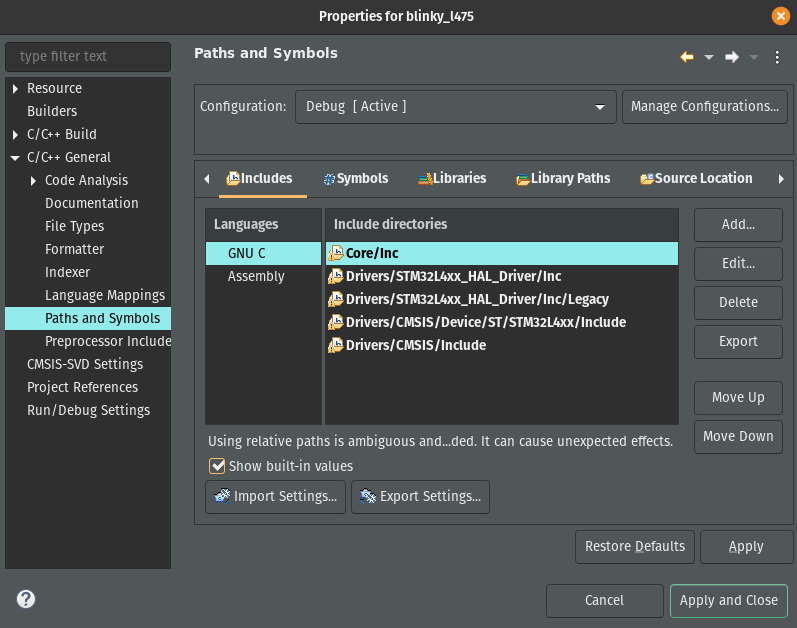
\includegraphics[scale=.4]{images/def_inc.png}
\caption{Included paths and defined symbols in project}
\label{fig:def_inc}
\end{figure}

\paragraph{LDFLAGS} The variable \verb|LDSCRIPT| contains the path of the linker script needed to link our project. STM32CubeIDE generates a linker script after the creation of the project, in the next section we will examine how to edit this linker script in order to create a Fortified Application.

\paragraph{Finishing up}
The remaining sections contain the rules used to compile and link together the application. Under normal use they do not require any editing.

At this point it is important to delete all the content of the Debug folder (except for the newly edited makefile) and test that the customized build process is fully functional by rebuilding the application.

\subsubsection{Linker Script Editing}
The linker script is the glue that ties together our application telling the compiler where the different functions and variables must go.
Since part of the RAM and flash memory are reserved for exclusive use of the Microvisor we need to alter it in order to place the Fortified Application at a specific location where the Microvisor will search.

After the initial configuration of the prject STM32CubeIDE generated two linker scripts: \textit{STM32L475VGTX\_FLASH.ld} and \textit{STM32L475VGTX\_RAM.ld}. In reality even the automatic build process uses only the first one, the second can be deleted.

In particular in \textit{STM32L475VGTX\_FLASH.ld} we need to edit the section cotaining the memory map in order to make it compatible with the one used by MCU-Fortifier. To do this, open the file and edit the code in Listing \ref{lst:linker_original} as shown in Listing \ref{lst:linker_mod}.

\begin{lstlisting}[caption={Original memory map of linker script},captionpos=b,label=lst:linker_original]
MEMORY
{
	RAM    (xrw)    : ORIGIN = 0x20000000,   LENGTH = 96K
	RAM2    (xrw)    : ORIGIN = 0x10000000,   LENGTH = 32K
	FLASH    (rx)    : ORIGIN = 0x8000000,   LENGTH = 1024K
}
\end{lstlisting}


\begin{lstlisting}[caption={New memory map compatible with MCU-Fortifier},captionpos=b,label=lst:linker_mod]
MEMORY
{
	FLASH (rx)                 : ORIGIN = 0x08021000, LENGTH = 0xdf000
	RAM (xrw)                  : ORIGIN = 0x20000040, LENGTH = 0x17FC0
	RAM2 (xrw)                 : ORIGIN = 0x10000000, LENGTH = 32K
}
\end{lstlisting}
The complete memory map used by MCU-Fortifier can be found in the file \textit{memory\_map.ld} included in the release. Listing \ref{lst:linker_mod} shows a simplified version where some of the entries have been removed (as they are not used by the Fortified Application). Another way to perform the modification of the linker script is to copy the file \textit{memory\_map.ld} in the same folder containing \textit{STM32L475VGTX\_FLASH.ld}, then removing the memory map section from the latter one and replacing it with the directive ``\verb|INCLUDE memory_map.ld|'' which will automatically include the content of \textit{memory\_map.ld}. When using this second method, make sure that the name of the different memory areas (e.g. \verb|FLASH|, \verb|RAM|) correspond to the ones used in the linker script.

\subsection{Customize Debug Process}
Now the application fotification process is completed. In order to debug the fortified application we need the debugger in order to correctly load all the necessary information froth both the Micorvisor executable (\textit{MCU-Fortifier.elf}) and the application executable (\textit{blinky\_l475.elf}).
Furthermore we also need to flash the both of them on the device, this can be done in different ways:
\begin{itemize}
	\item Using STM Cube IDE.
	\item Using the STM dedicated utility: STM32 Cube Programmer.
	\item Through the OTA capabilities of MCU-Fortifier, downloading the fortified application from the Update Server.
\end{itemize}
It's important to remember that flashing an application to the device flash memory does not erase all of the flash content. Instead only the memory address that are explicitly flashed are modified while the remaining memory retains previously written content.

In our following example we will configure STM Cube IDE to flash both the Microvisor and Fortified application each time the \textit{Debug} button is pressed. To do so, right click on the project, select \textit{Debug As} and click on \textit{Debug Configurations...}.

Open the \textit{Startup} tab, now we need to add to the list the Microvisor executable by clicking on \textit{Add} and browsing the file system to the location where it is stored (the process to obtain the Microvisor executable is outlined in Section \ref{sec:microvisor_compile}).

Ensure that the Microvisor executable is the last item on the list, before its file name a green play button should appear as depicted in Figure \ref{fig:startup}. This ensures that it will be the first code executed on boot, otherwise the fortified application would be executed directly without performing all the necessary configuration steps and resulting in unpredictable behaviors.

\begin{figure}
\centering
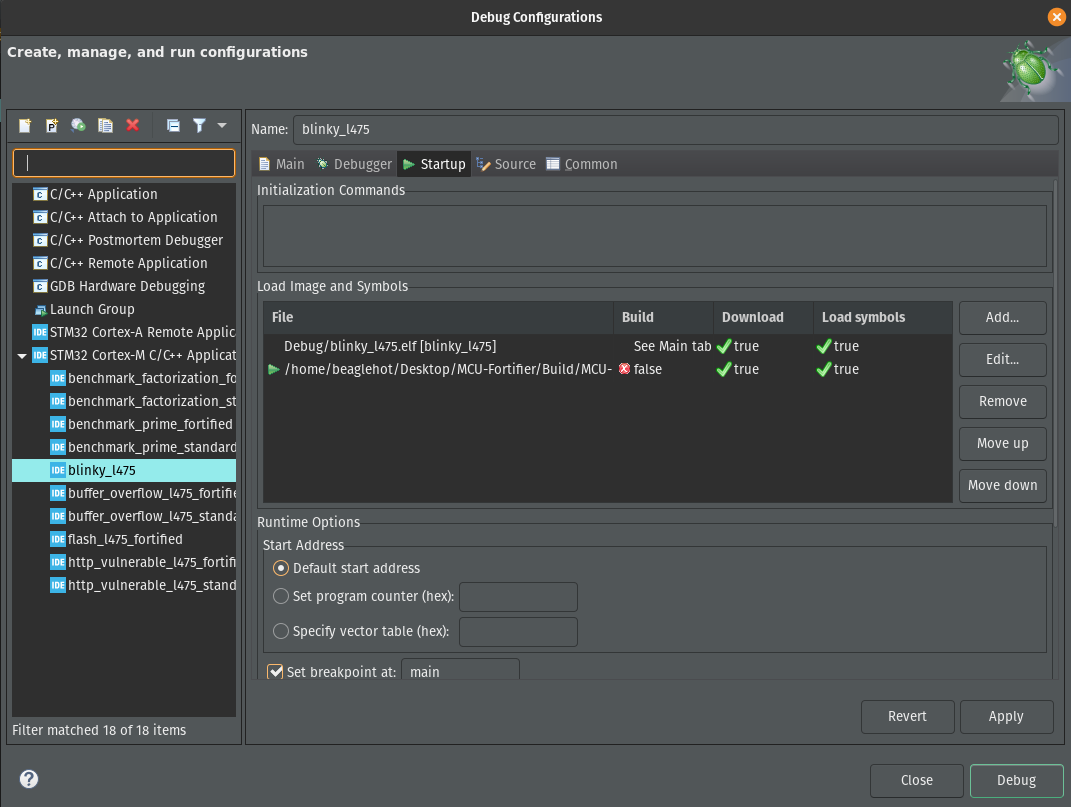
\includegraphics[scale=.32]{images/startup.png}
\caption{Project debug configuration}
\label{fig:startup}
\end{figure}

While in the \textit{Startup} tab, make sure to uncheck the option ``\textit{Halt on exception}'' as they are often triggered by the Microvisor as a way to monitor the application. Leaving this option on would interfere with the debugging process, resulting in constant halting of the code.

Now the Fortified Application can be executed via a normal debug session. The debugger ensures that both the Fortified Application and Microvisor executables will be flashed on the board. On boot the board will start executing the Microvisor which will perform the basic configuration operation and bootstrap the execution of the application.
By starting a new Debug session the leds on the board should now start blinking (after the Microvisor has been correctly activated).

\subsection{Source Code Modification}
In specific source files (e.g. the startup code) are present directives that instruct on what processor to target during the build process. STM32CubeIDE automatically detects the B-L475E-IOT01A1 board as having a Cortex-M4 processor and inserts directives such as \verb|.cpu cortex-m4|. Since MCU-Fortifier is designed to work with Cortex-M3 devices (which only support a subsection of Cortex-M4 instructions) and the correct architecture is already specified with command line options, we must delete all these directives (e.g. using a single search-and-replace).


\subsection{Restrictions on Fortified Application}
Due to the design of MCU-Fortifier and the fact that Fortified Applications run always in unprivileged mode, there are some restriction on how Fortified Application can be developed:
\begin{itemize}
    \item Interrupt handlers (as the rest of the code) always run without privileges and cannot access the content of the stack prior to exception entry. Consequently the handler for SVC instructions cannot recover the SVC number from the stack, instead the Microvisor takes care of passing it as a parameter. The function signature for the SVC handler must be modified to accomodate this (e.g. \verb|SVC_Handler(int SVCnum)|).
    \item MCU-Fortifier does not currently support application based on other OS (e.g. MbedOS, FreeRTOS) as they perform context switch using interrupt that violate the previous constraint.
    \item All applications source files must be compiled with the instrumentation in order to handle system instructions (e.g. CPS, MRS, MSR) and other specific instructions. Failing to do so will result in an application that may malfunction.
    \item The Vector Table must always be stored at the beginning of the Fortified Application, meaning the lowest address of the flash portion reserved for the Fortified Application (by default STM32CubeIDE already takes care of this).
\end{itemize}

\section{Update Server}
The release of MCU-Fortifier comes equipped with a remote Update Server that, when properly configured, can be used to update remotely and securely the fortified user application of a board running the MCU-Fortifier Microvisor as well as the Microvisor itself.

Boards and Update Server communicate in a typical client-server model, furthermore the communication is encrypted and authenticated through the use of an AEAD Scheme (Authenticated Encryption with Associated Data) using Chacha20 and Poly1305.

\subsection{Communication Protocol}
The Update Server is a application that executes on a more powerful platform (such an x86\_64 computer) and passively waits for connections from the boards.
The typical communication protocol is shown in Figure \ref{fig:comm_proto} and works as follow:
\begin{enumerate}
	\item After boot, the Microvisor attempt to create an secure connection to the Update Server using the symmetric encryption key specified in the configuration. If the connection fails, the whole update process is skipped and the Microvisor starts executing the user application.
	\item After the connection has been established, if there are any error to report, the board proceeds ot report them otherwise this step is skipped.
	\item The Microvisor checks for update regarding its own code. If there are, it proceeds to download them and reboot the board otherwise this step is skipped. \textbf{Attention}: Updating the Microvisor will automatically delete any fortified application previously installed!
	\item The Microvisor then computes an hash of the fortified user application currently stored on board and sends it to the server asking if there are any updates. The Update Server compares the received hash with the one of the latest update available for that fortified application. If they do not match the server replies with a message indicating that an update is indeed available.
	\item If an update is available, the Microvisor deletes the previous application from flash and starts the update process by asking the size of the update and then repeatedly asking the server for small chunks of data which are flashed in memory as they are received. After all the data has been received, the Microvisor computes a new hash of the user application and verifies if the update was successful by querying the server for more updates.
	\item After all the communication steps have been performed, the connection is closed and the Microvisor proceeds to boot the fortified user application (only the board has been activated).
\end{enumerate}

\begin{figure}
	\centering
	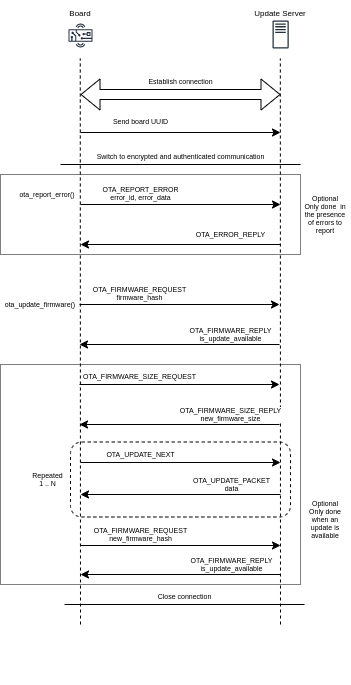
\includegraphics[scale=.77]{images/comm_proto.png}
	\caption{Communication protocol between board and update server}
	\label{fig:comm_proto}
\end{figure}

\subsection{Error Reporting}
Beyond using the remote server for update, the Microvisor also uses it to report errors that are encountered during the execution. In fact after an unrecoverable error occurs, the Microvisor logs it to flash and reports the error encountered on the next connection to the server.

It is important to keep in mind that the communication with the Update Server happens immediately after boot and before the fortified application is started. The Microvisor cannot communicate with the Update Server while the fortified application is running. This is mainly due to 2 reasons:
\begin{itemize}
	\item The communication stack requires the peripherals to be reinitialized therefore losing the state in which the fortified application left them.
	\item The communication stack requires a lot of RAM which is often not available because already used by the fortified application.
\end{itemize}

\subsection{Configuring Update Server}
As of Revision 1.2 the server consists of a simple python script that can be executed on any machine with an internet connection. In particular the script \textit{start\_server.py} contained in the folder \textit{UpdateServer} can be used to setup the SSL server. Inside of it there are different variables that can be modified to adapt the configuration, in particular:
\begin{itemize}
	\item \verb|SERVER_IP| is a string containing the IP of the network interface used by the server\footnote{If the server is behind a NAT additional configuration will be required on the NAT in order to forward packets correctly to the server IP.}.
	\item \verb|SERVER_PORT| port used by the server.
	\item \verb|uuid_key_map| dictionary in the form $(uuid:key)$. Used to associate a board UUID with the relative symmetric encryption key used to encrypt and authenticate the communication.
	\item \verb|uuid_firmware_map| dictionary in the form $(uuid:firmware)$. Used to associate a board UUID with the latest version of its fortified user application so that during boot the board will perform an update if necessary. To configure a new update, simply add the UUID of your board and the path to the desired binary file.
	\item \verb|uuid_microvisor_map| dictionary in the form $(uuid:microvisore)$. Used to to associate a board UUID with a Microvisor update.
\end{itemize}
The \textit{binaries} folder contains 3 binary files:
\begin{itemize}
	\item \verb|blink_l475_green.bin| pre-compiled binary of the \textit{blink\_l475} application, toggles green led.
	\item \verb|blink_l475_network.bin| pre-compiled binary of the \textit{blink\_l475} application, toggles network led (yellow and blue).
\end{itemize}

\end{document}
